\documentclass[hyperref=colorlinks]{beamer}
\mode<presentation>
\usetheme{iclpt}
\setbeamertemplate{navigation symbols}{}
\setbeamertemplate{headline}{
  \begin{beamercolorbox}[leftskip=.2cm,rightskip=.2cm,topskip=.2cm,ht=1.1cm,dp=0.1cm,wd=\textwidth]{institute in head/foot}
    
\includegraphics[height=1cm]{icl.pdf}
    \hfill
%    \includegraphics[height=1cm]{../Pics/ATLAS-Logo-Square-Blue-RGB.png}
%    
\includegraphics[height=1cm]{../Pics/CMS-Color.pdf}
    
\includegraphics[height=1cm]{TalkPics/t2k_logo_large.png}

%??put t2k logo here
  \end{beamercolorbox}
}
\setbeamertemplate{footline}{
  \begin{beamercolorbox}[ht=.35cm,dp=0.2cm,wd=\textwidth,leftskip=.3cm]{author in head/foot}%
    \begin{minipage}[c]{5cm}%
      \usebeamerfont{author in head/foot}
      \insertshortauthor 
      \insertshorttitle
    \end{minipage}\hfill%
    \hfill
    \insertframenumber{} / \ref{lastframe}
    %\hfill
    \begin{minipage}{6cm}
      \hfill
      %\insertshorttitle
    \end{minipage}
  \end{beamercolorbox}%
}

\definecolor{beamer@icdarkblue}{RGB}{0,51,102}
\definecolor{beamer@icmiddleblue}{RGB}{0,82,150} 
\definecolor{beamer@iclightblue}{RGB}{200,212,232}
\definecolor{beamer@icmiddlered}{RGB}{204,51,0}
\definecolor{beamer@iclightred}{RGB}{232,212,32}

\usepackage{tikz}
\usetikzlibrary{arrows,shapes,backgrounds}
\usepackage{color}
\usepackage{tabularx,colortbl}
\usepackage{graphicx}
\usepackage{pdfpages}
\usepackage{feynmp}
\usepackage{rotating}
\usepackage{moresize}
\usepackage{slashed}
\usepackage{xcolor,colortbl}
\DeclareGraphicsRule{*}{mps}{*}{}
\hypersetup{colorlinks=false}

\title[Asimov comparisons with different dcp values]{\vspace{-0.2cm} Asimov comparisons with different dcp values}
\author[P. Dunne]{Patrick Dunne - Imperial College London}
\titlegraphic{
  \vspace{-0.4cm}
}
\date{}
\begin{document}
\tikzstyle{every picture}+=[remember picture]
\tikzstyle{na} = [baseline=-.5ex]
\begin{fmffile}{t2ktemplatefeyndiags}


  %TITLE PAGE
  %20 mins + 5 questions
  \section{Title}
  \begin{frame}
    \titlepage
  \end{frame}

  \begin{frame}
    \frametitle{Overview}
    \begin{block}{}
      \begin{itemize}
      \item Asked to study three new Asimov points by OA
      \item All based on point 1/A but with different values of dcp (see below)
      \item 1M steps generated for each point woRC
      \end{itemize}
      \centering
      \begin{tabular}{|l|c|c|c|c|}
        \hline
        Set & A & C & D & E \\
        \hline
        $\sin^2(\theta_{12})$ & \multicolumn{4}{c|}{0.304}\\
        $\sin^2(\theta_{13})$ & \multicolumn{4}{c|}{0.0217}\\
        $\sin^2(\theta_{23})$ & \multicolumn{4}{c|}{0.528}\\
        $\Delta m^2_{12}$ & \multicolumn{4}{c|}{7.35e-05}\\
        $\Delta m^2_{23}$ & \multicolumn{4}{c|}{0.002509}\\
        $\delta_{CP}$ & -1.601 & 0 & $\pi$ & $\frac{pi}{2}$ \\
        \hline
      \end{tabular}
    \end{block}
  \end{frame}

  \begin{frame}
    \frametitle{CP conserving sets - appearance parameters}
    \centering
    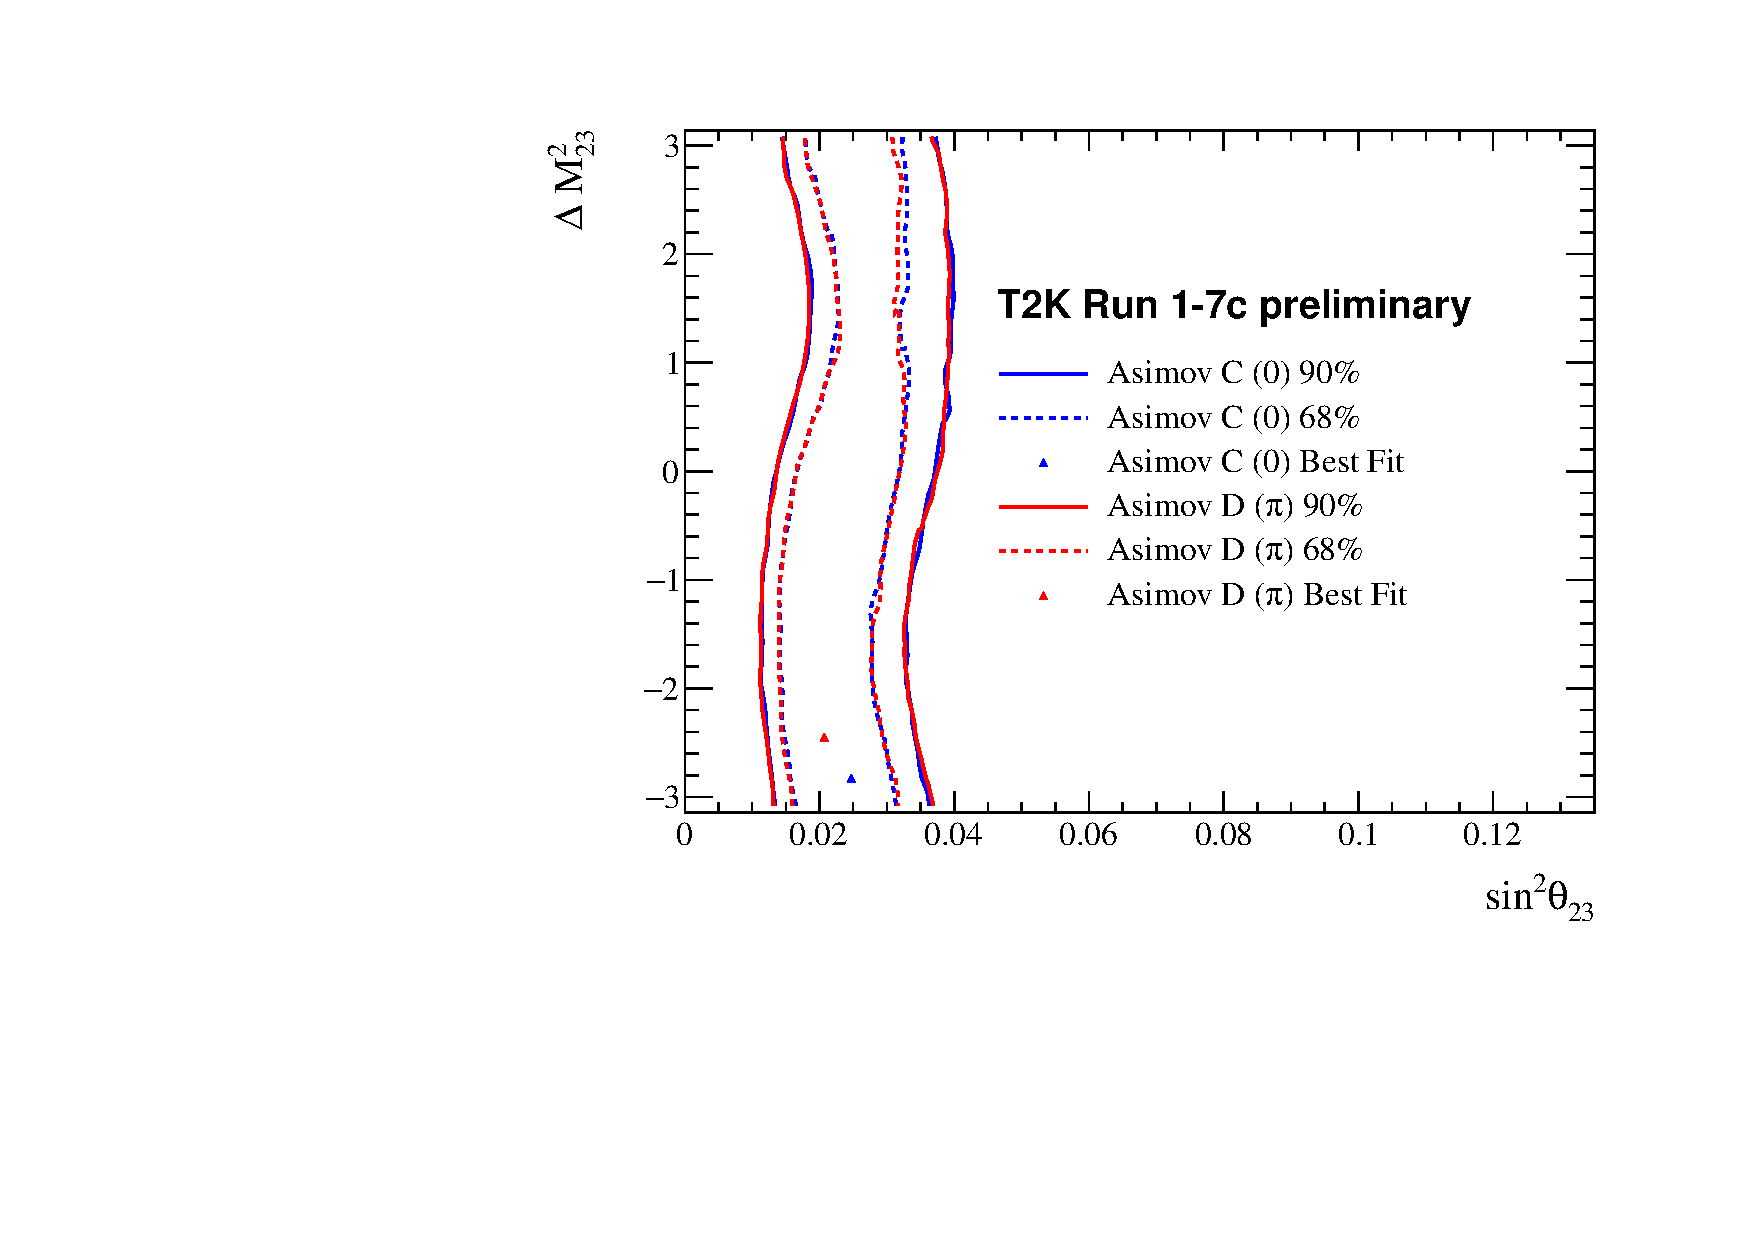
\includegraphics[width=.65\textwidth]{TalkPics/newasimovs_060916/contours_newasimovcomparisons_woRC_060916/comparedcontours_th13dcp_cpconservingasimovs_official.pdf}
  \end{frame}

  \begin{frame}
    \frametitle{CP conserving sets - disappearance parameters}
    \centering
    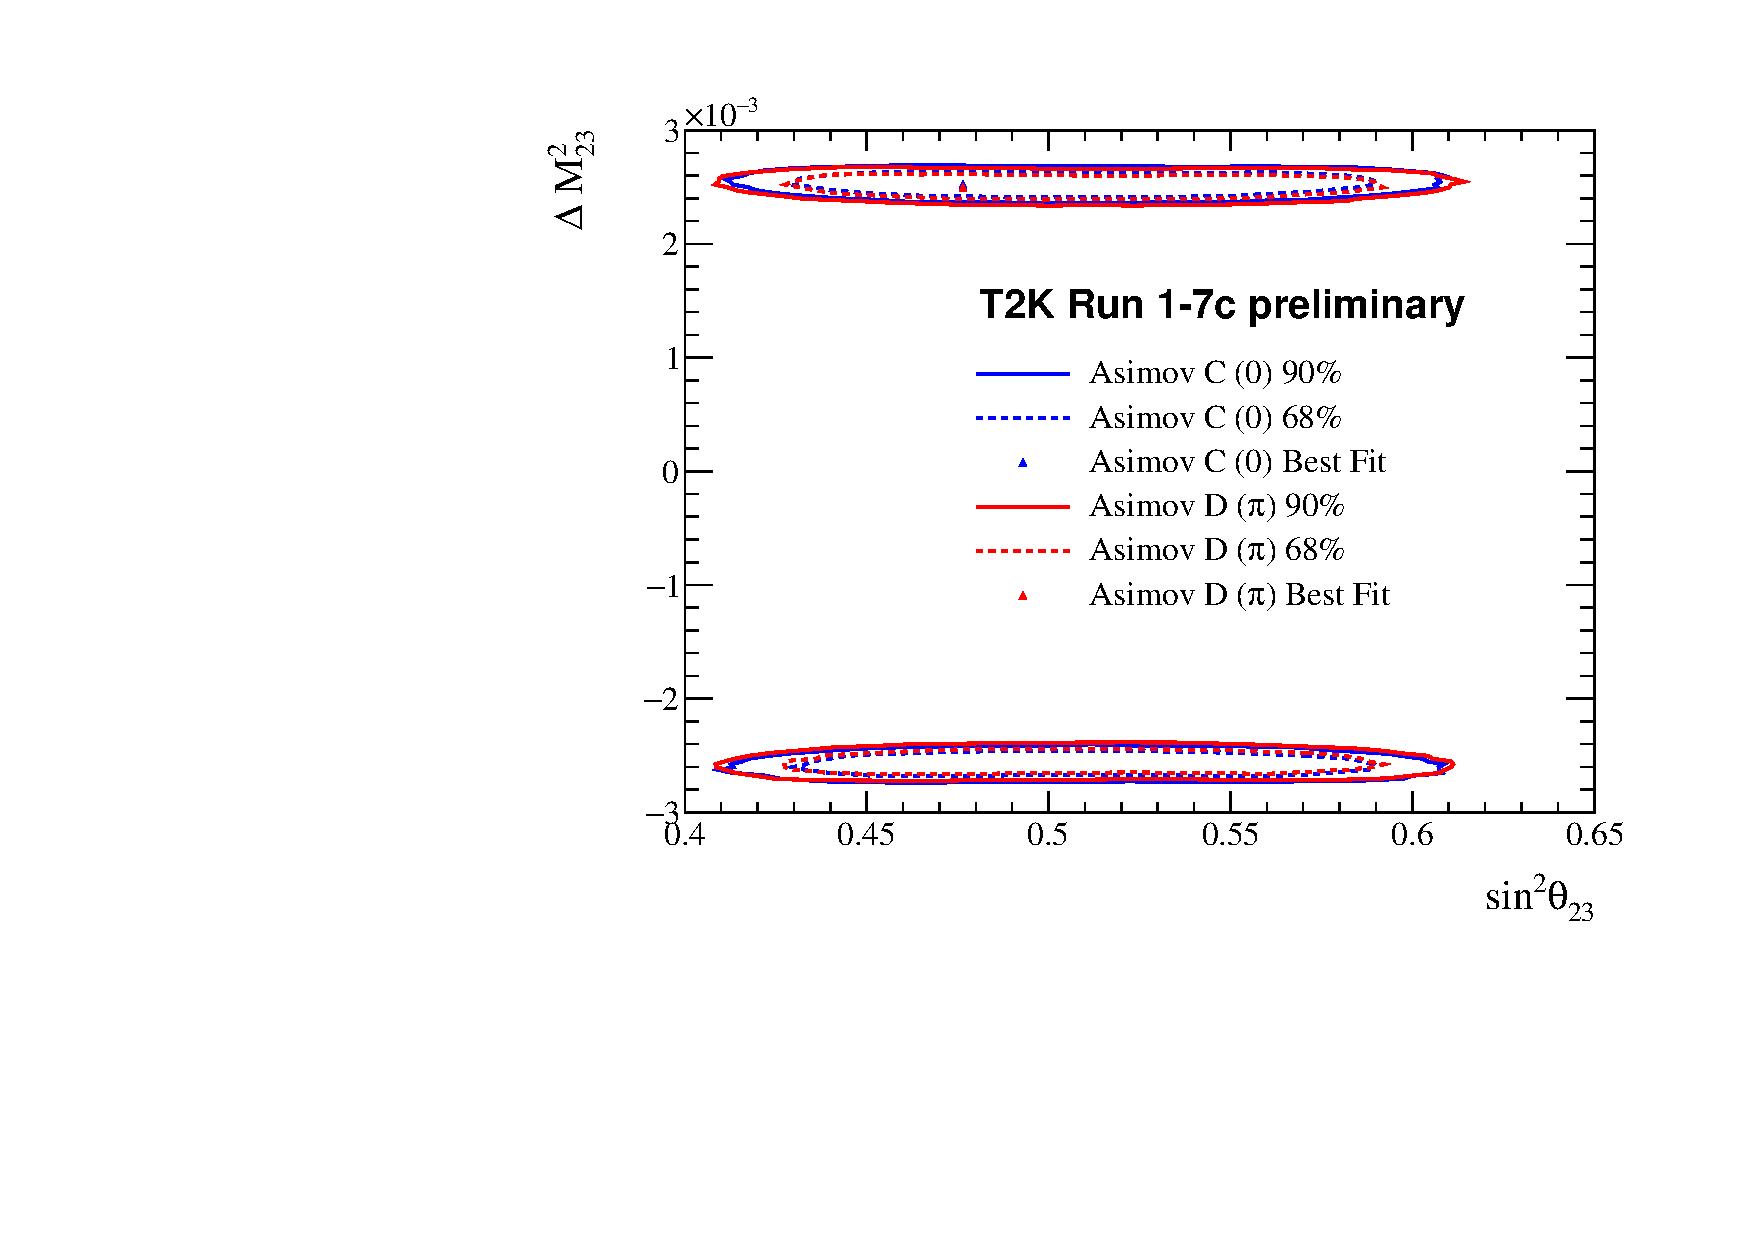
\includegraphics[width=.65\textwidth]{TalkPics/newasimovs_060916/contours_newasimovcomparisons_woRC_060916/comparedcontours_th23dm23_cpconservingasimovs_official.pdf}
  \end{frame}

  \begin{frame}
    \frametitle{CP conserving sets - dcp}
    \centering
    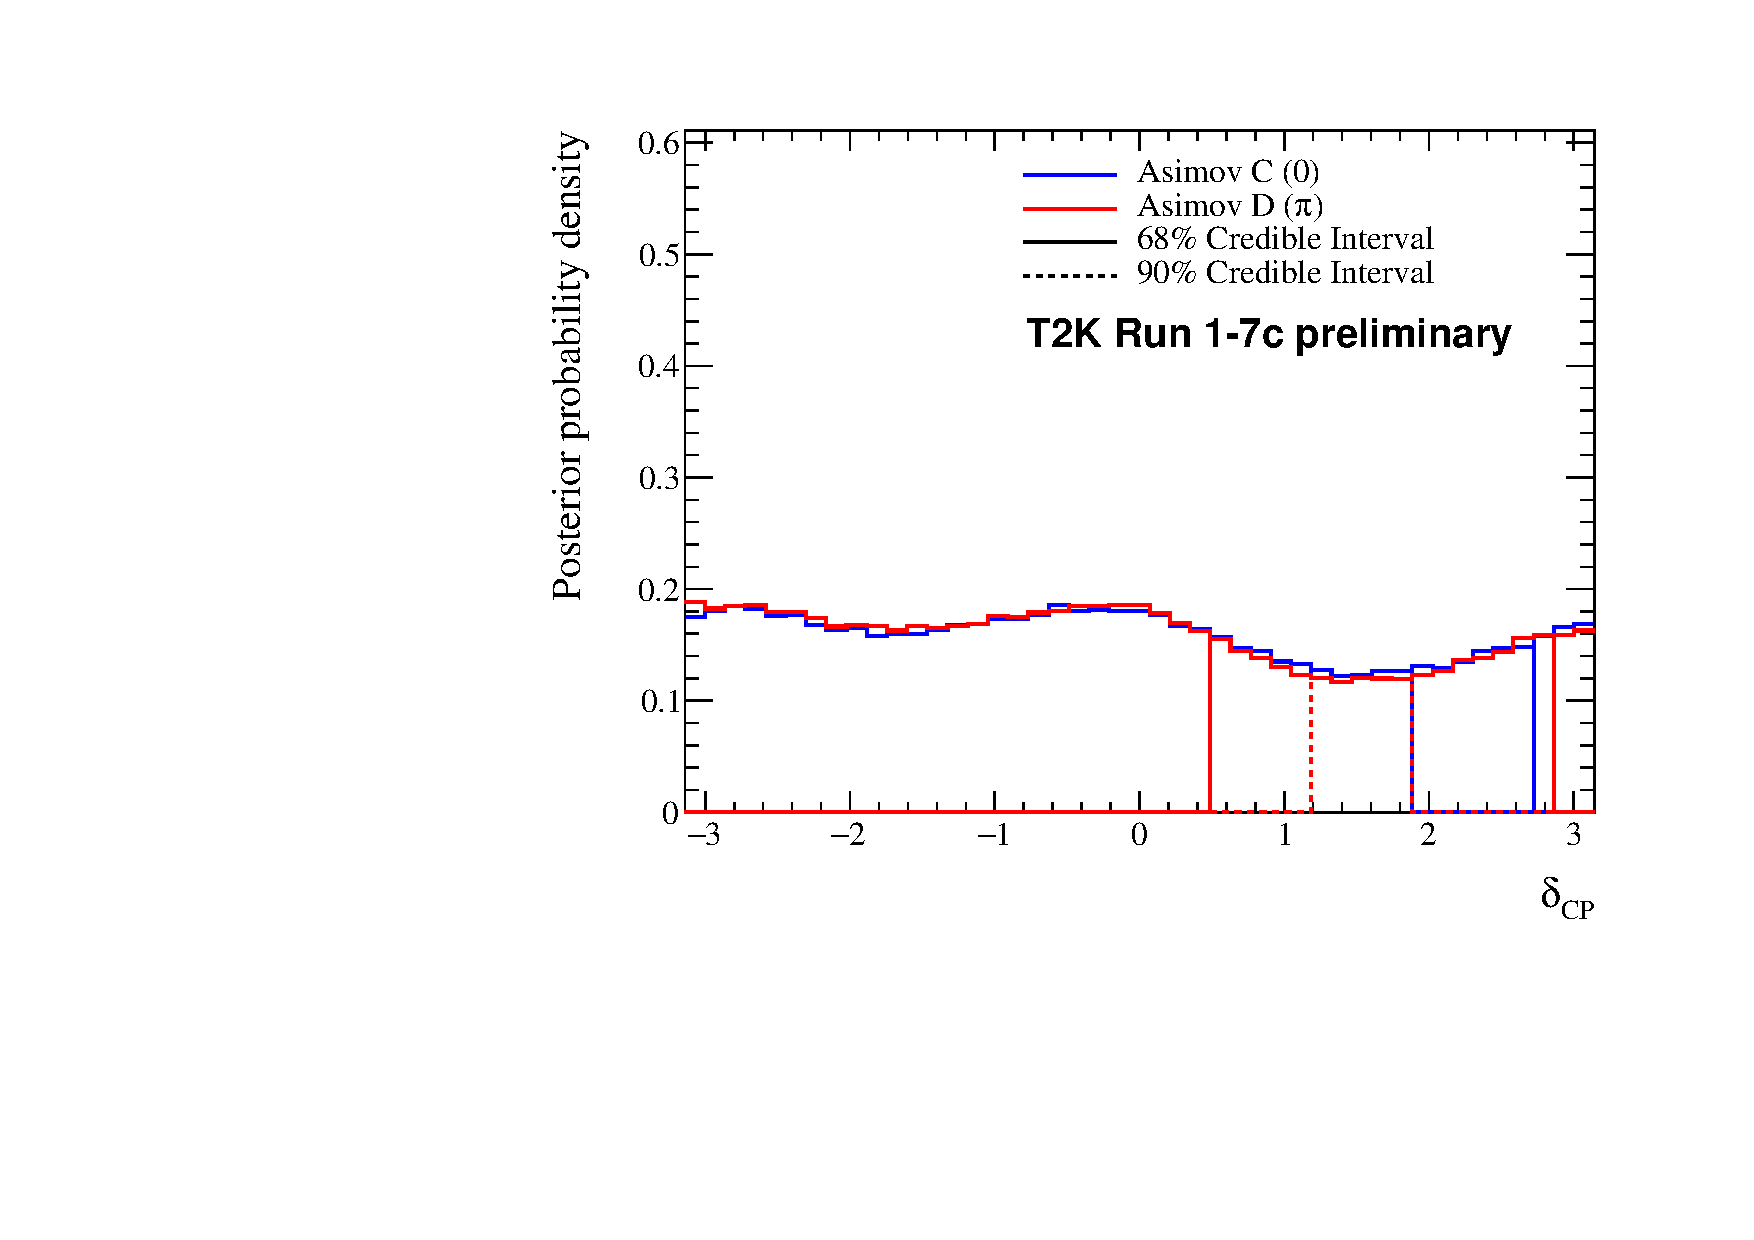
\includegraphics[width=.65\textwidth]{TalkPics/newasimovs_060916/contours_newasimovcomparisons_woRC_060916/contours_1D_dcp_cpconservingasimovs_compare_official.pdf}
  \end{frame}

  \begin{frame}
    \frametitle{CP violating sets - appearance parameters}
    \centering
    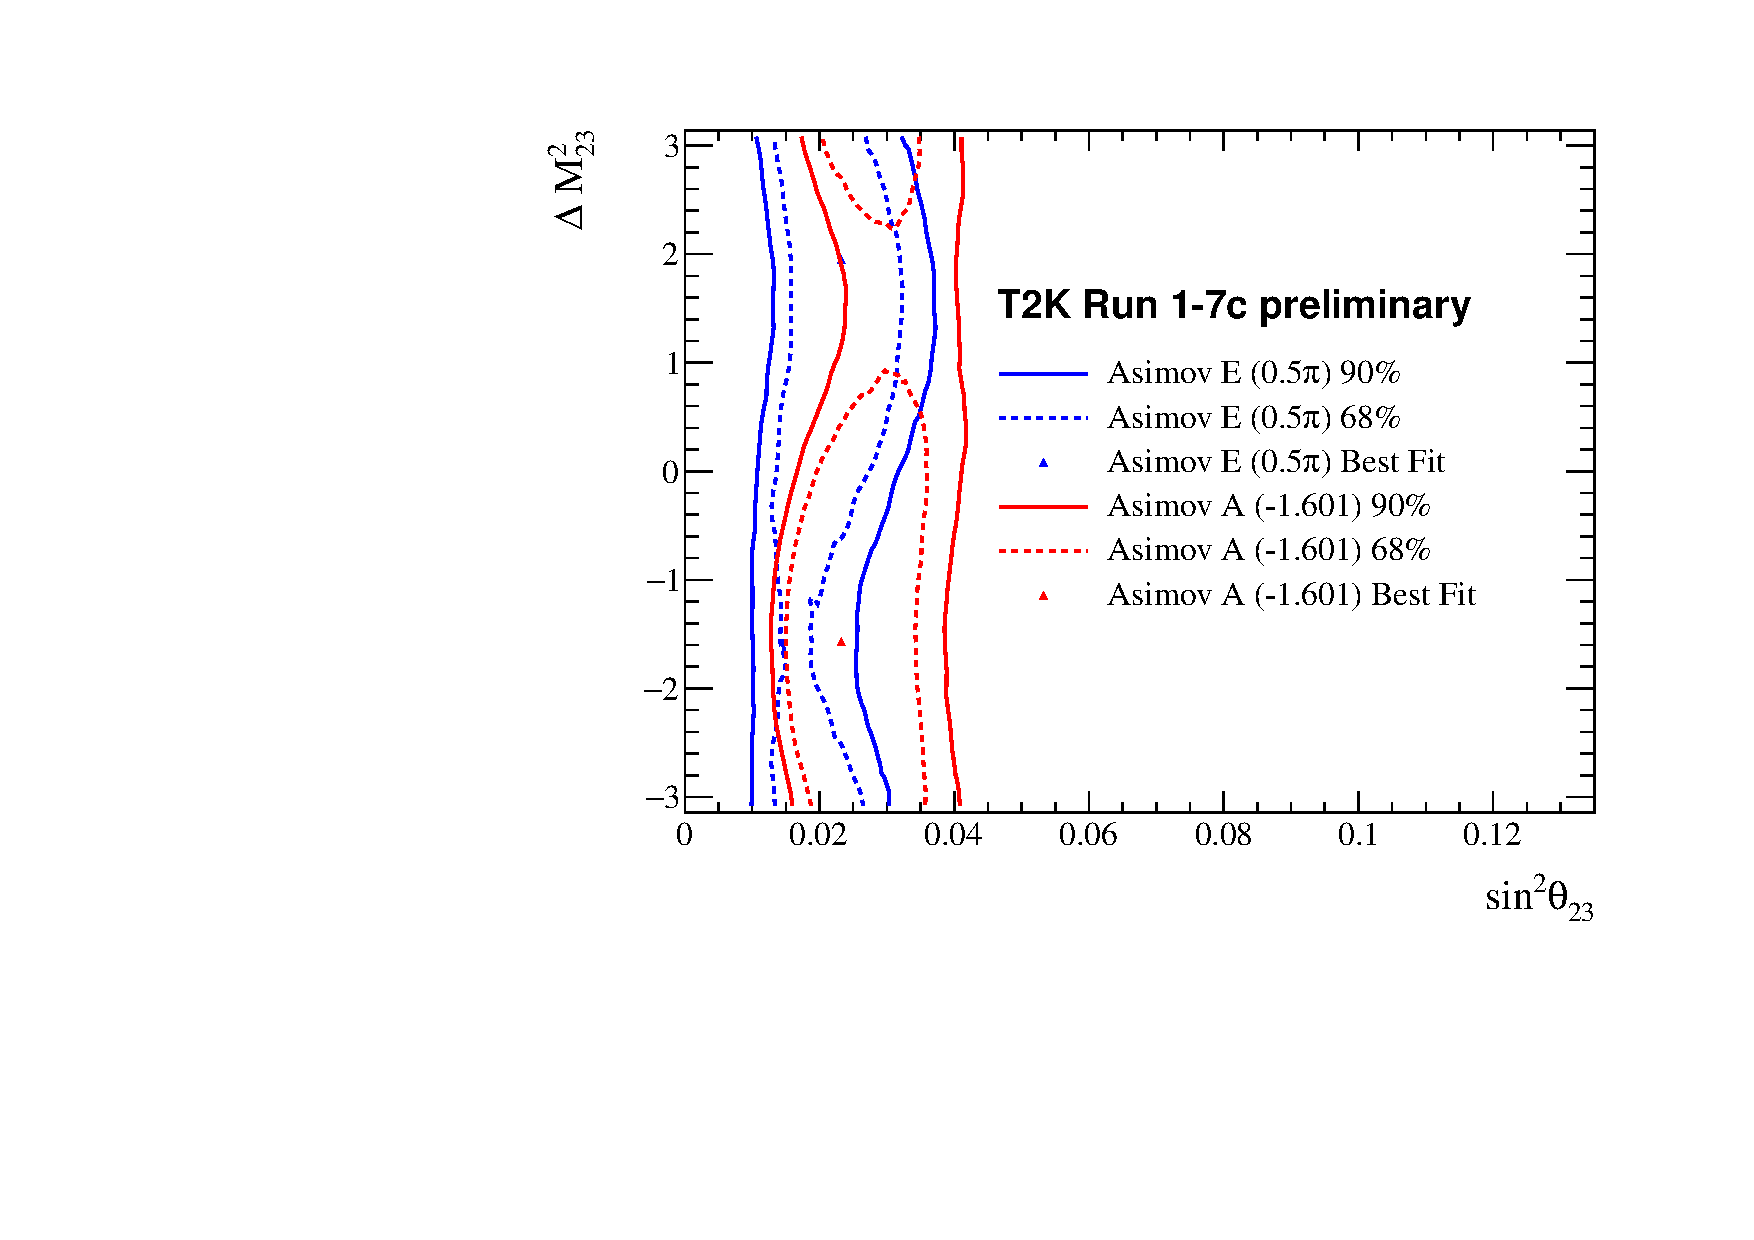
\includegraphics[width=.65\textwidth]{TalkPics/newasimovs_060916/contours_newasimovcomparisons_woRC_060916/comparedcontours_th13dcp_cpviolatingasimovs_official.pdf}
  \end{frame}

  \begin{frame}
    \frametitle{CP violating sets - disappearance parameters}
    \centering
    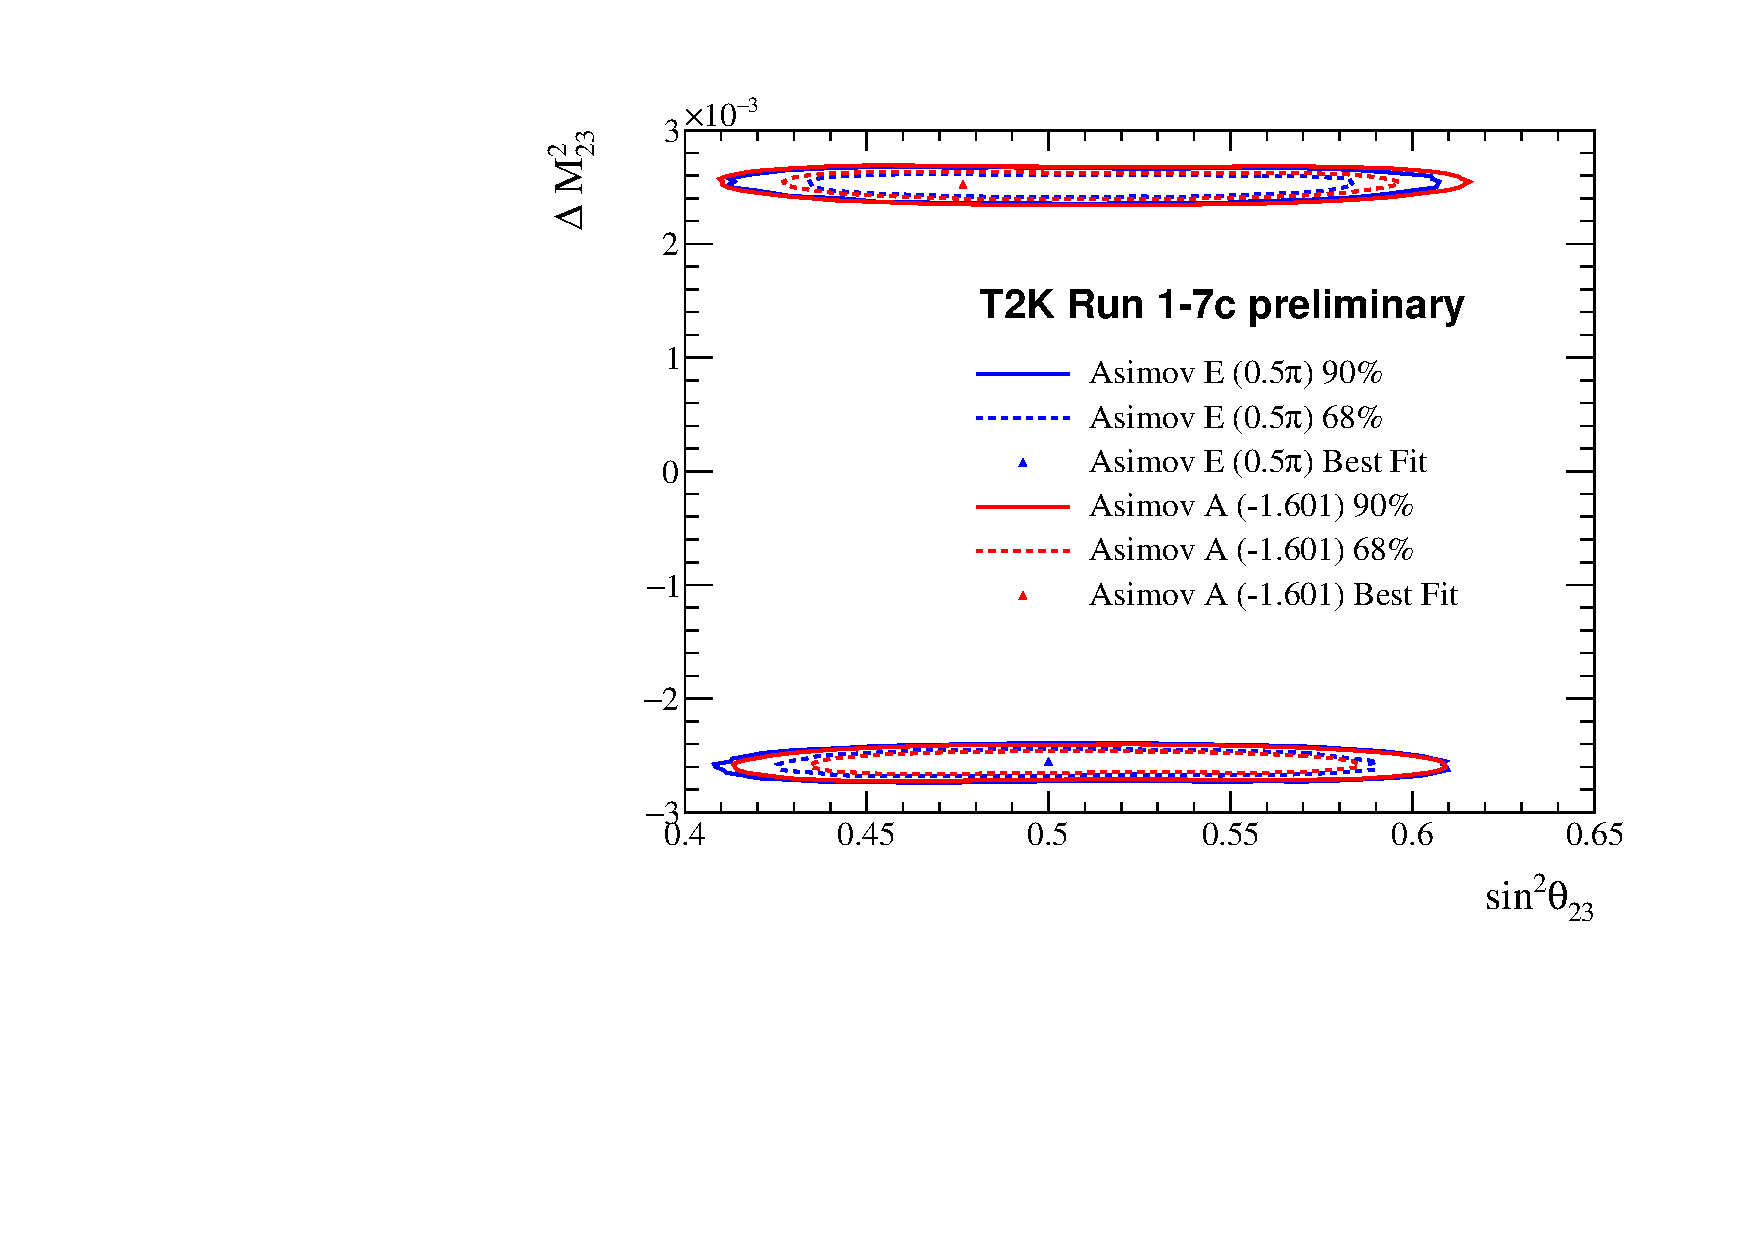
\includegraphics[width=.65\textwidth]{TalkPics/newasimovs_060916/contours_newasimovcomparisons_woRC_060916/comparedcontours_th23dm23_cpviolatingasimovs_official.pdf}
  \end{frame}

  \begin{frame}
    \frametitle{CP violating sets - dcp}
    \centering
    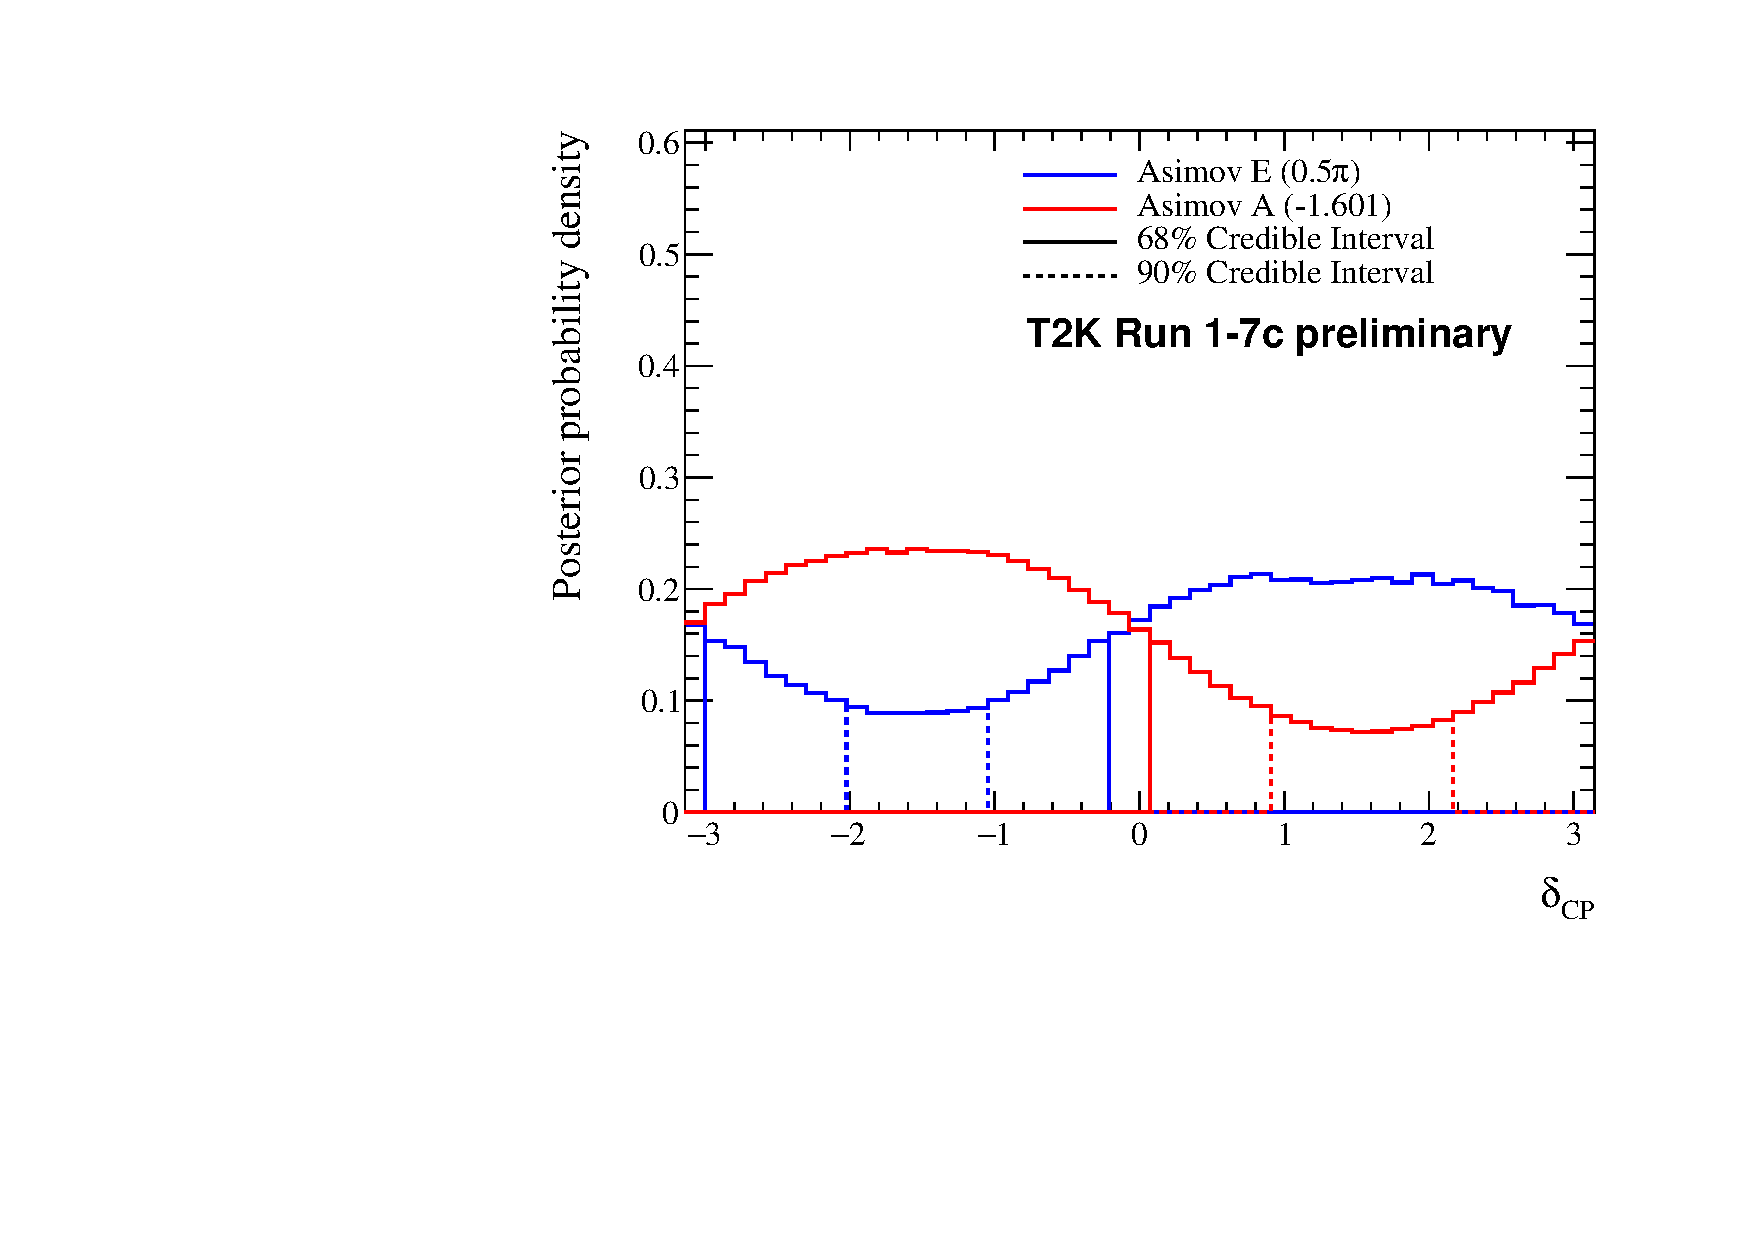
\includegraphics[width=.65\textwidth]{TalkPics/newasimovs_060916/contours_newasimovcomparisons_woRC_060916/contours_1D_dcp_cpviolatingasimovs_compare_official.pdf}
  \end{frame}





  \begin{frame}
    \frametitle{}
    \label{lastframe}
    \begin{block}{}
      \begin{itemize}
      \item Little difference between CP conserving asimovs
      \item CP violating Asimovs show tighter exclusions for -1.601 than pi by 2
      \item wRC being processed now
      \end{itemize}
    \end{block}
  \end{frame}

  %Backup goes here
  
\end{fmffile}
\end{document}

